% ====================
\chapter{Perceiving a Suitable Parking Spot}
% ====================

% • In a paper you MUST provide the details, but FIRST convey the idea
% • Introduce the problem, and your idea, using EXAMPLES and only then
% present the general case
% • Explain it as if you were speaking to someone using a whiteboard
% • Conveying the intuition is primary, not secondary
% • Once your reader has the intuition, she can follow the details (but not vice
% versa)
% Even if she skips the details, she still takes away something valuable
% Evidence
% • Your introduction makes claims; The body of the paper provides evidence to
% support each claim
% • Check each claim in the introduction, identify the evidence, and forward-
% reference it from the claim
% • Evidence can be: analysis and comparison, theorems, measurements, case
% studies

% ====================
\section{General Idea}
% ====================
We first address the problem of identifying a suitable parking spot for a
wheelchair in an indoor environment. The identified parking spot will then be
used as a goal state for a planner to subsequently move the robot to.

We start with the simple case of the following assumptions:
\begin{itemize}
\item We will use one RGB-D camera for detection
\item The algorithm will work in an indoor environment. Objects on the floor
will be: humans, chairs, other wheelchairs, tables and cabinets.
\item The floor will be flat throughout (i.e. no ramps)
\item The suitable parking spot in question is entirely viewable by the camera.
In practice this means the RGB-D camera is facing the parking spot such that
it is visible and it is not overshadowed by any obstacle.
\item a 2d occupancy map will be used
\end{itemize}

% Why not front and back cameras?

\begin{figure}
\centering
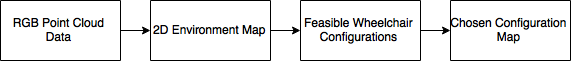
\includegraphics[width=3in]{figures/rgbdmap.png}
\caption{Pipeline}
\label{fig:rgbdmap}
\end{figure}

\autoref{fig:rgbdmap} shows the general pipeline.



% ====================
\section{Preprocessing the Point Cloud}
% ====================

To make a map, we are inspired by the approaches of Holz \cite{holz2013towards}
and Gritti \cite{gritti2014kinect} to detect obstacles based on their height
from the ground plane.

First, the point cloud is downsampled using a voxelized grid approach with a 1mm
grid filter. This reduces the computational load and prevents excess weighting of
certain volumes in the ground plane detection.

Next, a modified version of RANSAC is used to estimate the ground plane. This is
done for multiple reasons:
\begin{itemize}
\item Allows map to be taken relative to the ground plane
\item An obstacle can then be characterized by any point that resides above the
ground plane
\item Frame-by-frame plane detection is done for robustness to changing angles of
the camera.
\end{itemize}

Algorithm \autoref{alg:modifiedRansac} shows the modified version of RANSAC,
which results in a 4-tuple $(a,b,c,d)$ satisfying $ax + by + cz + d = 0$
representing the ground plane.

\begin{algorithm}
\caption{Modified RANSAC}
\label{alg:modifiedRansac}
\begin{algorithmic}[1]
\Require{
$k$ is the number of iterations to run, P are points in $\mathbb{R}^3$ with the
positive $y$ axis roughly vertical upwards, $\theta_{max}$ is the maximum
inclination angle, $t$ is the threshold used to identify if a point fits the
plane}
\Statex
\Function{ModifiedRANSAC}{$k, P, \theta_{max}, t$}
    \State $n \gets 3$, the minimum number of points to specify a plane
    \State $d \gets 0$, the number of points that lie on the current best plane
    \For{$k$ iterations}
        \State Draw a sample of $n$ non-collinear points from $P$ uniformly at random
        \State $l \gets$ the plane that includes all $n$ points
        \If{the angle between the x-z axis and plane $l$ is greater than $\theta_{max}$}
            \State the plane is too steep, continue to the next iteration
        \EndIf
        \State Find the subset of points $p \in P$ such that all points in $p$ are
        within distance $t$ from plane $l$
        \If{$|p| > d$}
            \State $bestPlane \gets l$, the current best ground plane candidate.
            \State $d \gets |p|$
        \EndIf
    \EndFor
    \State ensure $bestPlane$ has a positive $y$ coefficient ($b$) for consistency
\EndFunction
\Statex
\Ensure{$bestPlane$, a 4-tuple $(a,b,c,d)$ that satisfies $ax + by + cz + d =
0$ representing the ground plane}
\end{algorithmic}
\end{algorithm}

The coordinate system for the point cloud is then rotated so the resulting
ground plane is aligned with the x-y axis.

% ====================
\section{Generating a 2D Map}
% ====================
The 2D Map is generated by projecting the 3D ground-aligned point cloud 
Algorithm \autoref{alg:groundmapprojection} shows how the point cloud is
converted to 2D histograms of object and ground locations. A Gaussian blur with
a standard deviation of 0.7 is applied to filter out holes and include a safety
buffer, and binarized by thresholding at zero, resulting in a binary object map.
Similarly, the 2D ground histogram is binarized by first applying a Gaussian
blur with a standard deviation of 0.5 and thresholding at zero. Additionally, a
1m circle around the origin of the camera is assumed to be viable positions in
the ground map, which accounts for the minimimum range of the RGBD camera. In a
conservative fashion, any true pixels in the ground map that shares a true value
in the object map is set to false, making the set of ground pixels and object
pixels mutually exclusive. A third map is created for pixels that are not
classified as a ground or object; hence each pixel must be classified as either
on the ground plane, an object, or unknown.

\begin{algorithm}
\caption{Ground Map Projection}
\label{alg:groundmapprojection}
\begin{algorithmic}[1]
\Require{$P_{rotated}$, $gridStepSize$, $groundThreshold$}
\Statex
\Function{GroundMapProjection}{$P_{rotated}, gridStepSize, groundThreshold$}
    \State $groundMap$, a 2D Histogram with bins spaced $gridStepSize$ metres apart
    \State $objectMap$, a 2D Histogram with bins spaced $gridStepSize$ metres apart
    \For{each point $p \in P_{rotated}$}
        \State $(x,y,z) \gets p$
        \If{$z < groundThreshold$}
            \State add $1$ to the appropriate $groundMap$ bin based on $(x,y)$
        \Else
            \State add $1$ to the appropriate $objectMap$ bin based on $(x,y)$
        \EndIf
    \EndFor
    \State $objectMap \gets GaussianBlur(objectMap, \sigma_1)$
    \State $objectMap \gets 1$ for each non-zero bin, $0$ otherwise

    \State $groundMap \gets GaussianBlur(groundMap, \sigma_2)$
    \State $groundMap \gets 0$ for each bin equal to zero and not already in $objectMap$, $1$ otherwise
\EndFunction
\Statex
\Ensure{$groundMap$, a 2D boolean array with values of $1$ representing the
ground, and $objectMap$}, a 2D boolean array with values of $1$ representing
impassible objects.
\end{algorithmic}
\end{algorithm}

% ====================
\section{Finding Feasible Parking Configurations}
% ====================
Three checks: If configuration can be fully placed on ground, if configuration
is reachable from the initial position, and if the cofiguration is not fully cut
off.
Algorithm \autoref{alg:feasibilitycheck} shows this.

\begin{algorithm}
\caption{Feasibility Check}
\label{alg:feasibilitycheck}
\begin{algorithmic}[1]
\Require{$groundMap$, $objectMap$}
\Statex
\Function{GroundMapProjection}{$P_{rotated}, gridStepSize, groundThreshold$}
    \State $groundMap$, a 2D Histogram with bins spaced $gridStepSize$ metres apart
\EndFunction
\Statex
\Ensure{$groundMap$, a 2D boolean array with values of $1$ representing the
ground, and $objectMap$}, a 2D boolean array with values of $1$ representing
impassible objects.
\end{algorithmic}
\end{algorithm}

% ====================
\section{Choosing a Suitable Parking Configuration}
% ====================
We don't have enough data.
Rely on heuristics.

Sum of squared closest distances


\begin{algorithm}
\caption{Potential Function Choice}
\label{alg:potentialfunctionchoice}
\begin{algorithmic}[1]
\Require{$groundMap$, $objectMap$}
\Statex
\Function{GroundMapProjection}{$P_{rotated}, gridStepSize, groundThreshold$}
    \State $groundMap$, a 2D Histogram with bins spaced $gridStepSize$ metres apart
\EndFunction
\Statex
\Ensure{$groundMap$, a 2D boolean array with values of $1$ representing the
ground, and $objectMap$}, a 2D boolean array with values of $1$ representing
impassible objects.
\end{algorithmic}
\end{algorithm}


% ====================
\chapter{Motion Planning}
% ====================
% --------------------
\section{Basic Ingredients}
% --------------------
\begin{itemize}
\item State
\item Time
\item Actions
\item Initial and Goal States
\item Feasibility and Optimality Criterion
\item A Plan
\end{itemize}

For a full description, see Chapter 1.3 of Lavalle \cite{lavalle2006planning}.
% --------------------
\section{Introduction to Motion Planning}
% --------------------
% --------------------
\subsection{Simple Motion Planning}
% --------------------
The simplest motion planning problems assume knowledge of a global map, a fixed
known goal state and a fixed known initial state. The problem is to determine a
feasible path from the initial state to the goal state. An optimality criterion
may also be applied to choose the best path if multiple feasible ones are found.

Notably, two important concepts have often been ignored in determining the path:
the differential constraints of the system and the use of feedback. Differential
constraints refers to how states transition to other states, and is inherent in
real-world systems, eg. a system's dynamics. For example, a car can easily move
fowards and backwards, but cannot immediately move side to side. Feedback refers
to the technique of refining further actions based on newly sensed data. In
simulations, feedback may not be necessary, but in real-world systems, errors in
sensing and modeling build up over time without it.

In this simple case, the generated path is followed in an open-loop manner, or
if subject to real-world constraints (see \autoref{fig:lavalle2006planning119}),
the generated path is smoothed to obey the system's dynamics and feedback is
used to closely follow the path. "Notably this approach is highly decoupled as
feedback and dynamics are neglected in constructing the original path"
\cite{lavalle2006planning}. The smooth path may now obey the robot's dynamics,
but may no longer be feasible.  Feedback is used merely as an inefficient
afterthought.

\begin{figure}
\centering
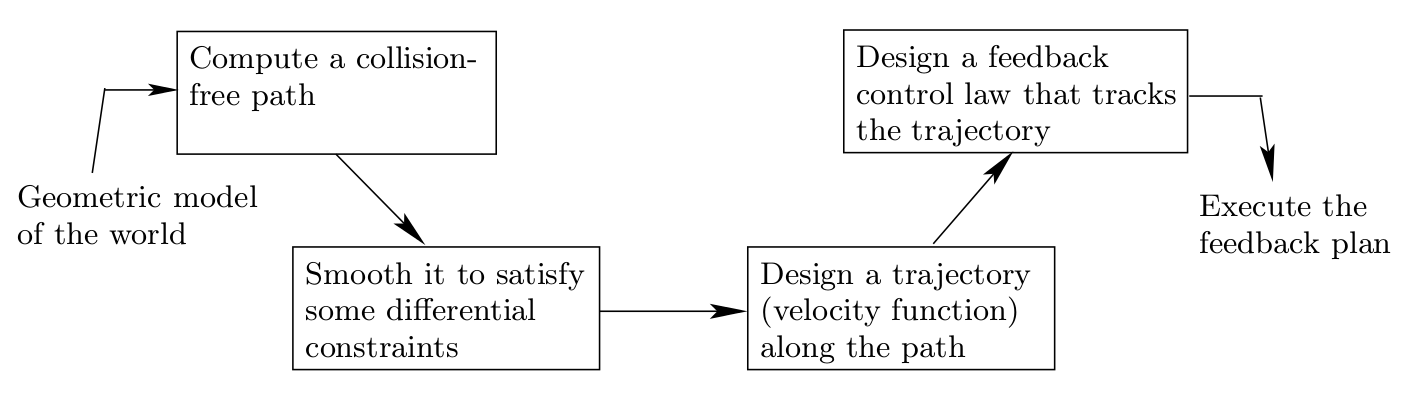
\includegraphics[width=3in]{figures/lavalle2006planning119.png}
\caption{From \cite{lavalle2006planning}. A refinement approach that has been used for decades in robotics.}
\label{fig:lavalle2006planning119}
\end{figure}

Even in this simple case, obtaining an optimal or even feasible path is not
straightforward if the state space is large. A* search for trivially sized state
spaces and sampling-based techniques such as RRTs (RRT* for optimality) and PRMs
have proven to be the methods of choice (citation?), though it is still an
ongoing field of interest (cite 2015 RRT/PRM papers).

% --------------------
\subsection{Feedback Motion Planning}
% --------------------
Dynamics refers, generally, to how a state transitions to another state.

Feedback (or reactive plans) refers to something else.

Tiers of motion planning problems
\begin{itemize}
\item Fixed Initial and Goal States, no dynamics, no feedback, some optimality
criterion: RRT*, PRM*
\item Fixed Initial and Goal States, dynamics, no feedback: RRT*, A*
\item Fixed Initial and Goal States, no dynamics, feedback
\end{itemize}

see \autoref{fig:determinedrive2}.

\begin{figure} % --------------------------------------
\centering
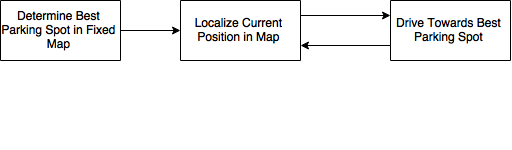
\includegraphics[width=3in]{figures/determinedrive2.png}
\caption{Feedback loop}
\label{fig:determinedrive2}
\end{figure}   % --------------------------------------


% --------------------
\subsection{Feedback Motion Planning with Updating Goal State}
% --------------------
see \autoref{fig:determinedrive1}.
For a full description, see Chapter 8 of Lavalle \cite{lavalle2006planning}.

\begin{figure} % --------------------------------------
\centering
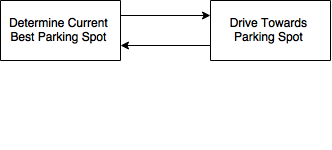
\includegraphics[width=3in]{figures/determinedrive1.png}
\caption{Feedback loop}
\label{fig:determinedrive1}
\end{figure}   % --------------------------------------

% --------------------
\section{Practical Options}
% --------------------
ROS Navigaiton Stack
http://www.dis.uniroma1.it/~nardi/Didattica/CAI/matdid/robot-programming-ROS-introduction-to-navigation.pdf

\begin{figure}
\centering
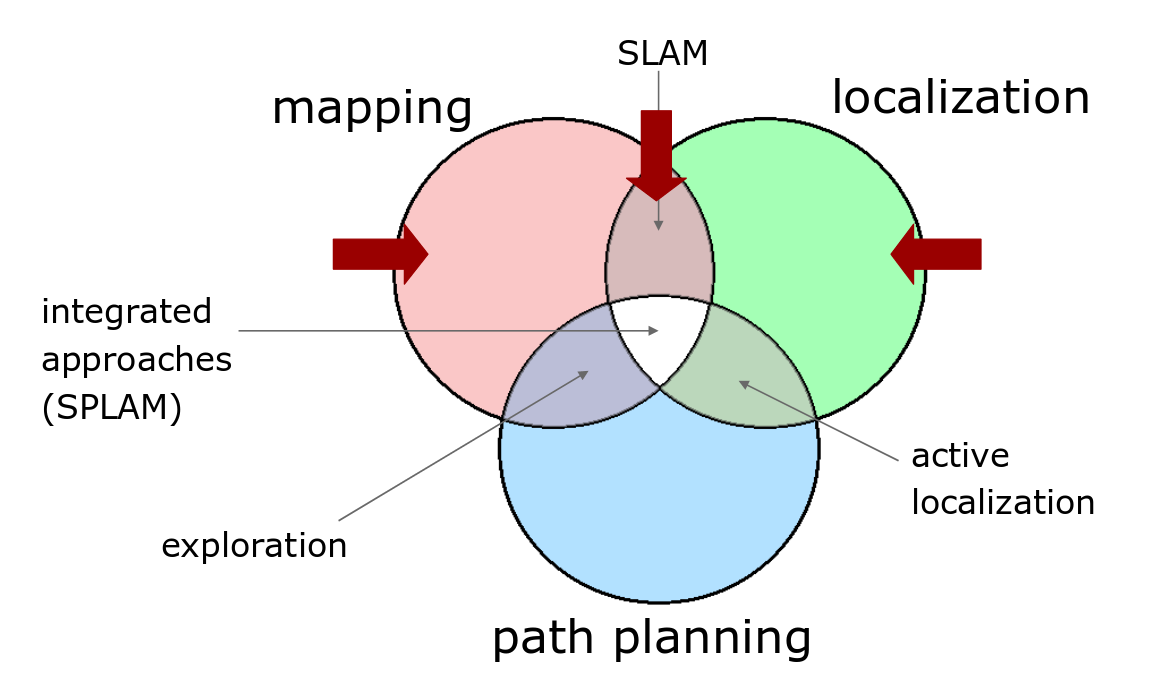
\includegraphics[width=3in]{figures/mappinglocalizationpathplanningvenndiagram.png}
\caption{Venn Diagram of Localization, Mapping and Path Planning}
\label{fig:mappinglocalizationpathplanningvenndiagram}
\end{figure}

We don't care about mapping
